\section{Lesson 5 -  The Blues scale}\\
\textbf{Blues Shuffle in G : Backing Track}\\
Practice lesson 4 along to this: \\ 
https://www.youtube.com/watch?v=o5xCVtkOPVc\\


    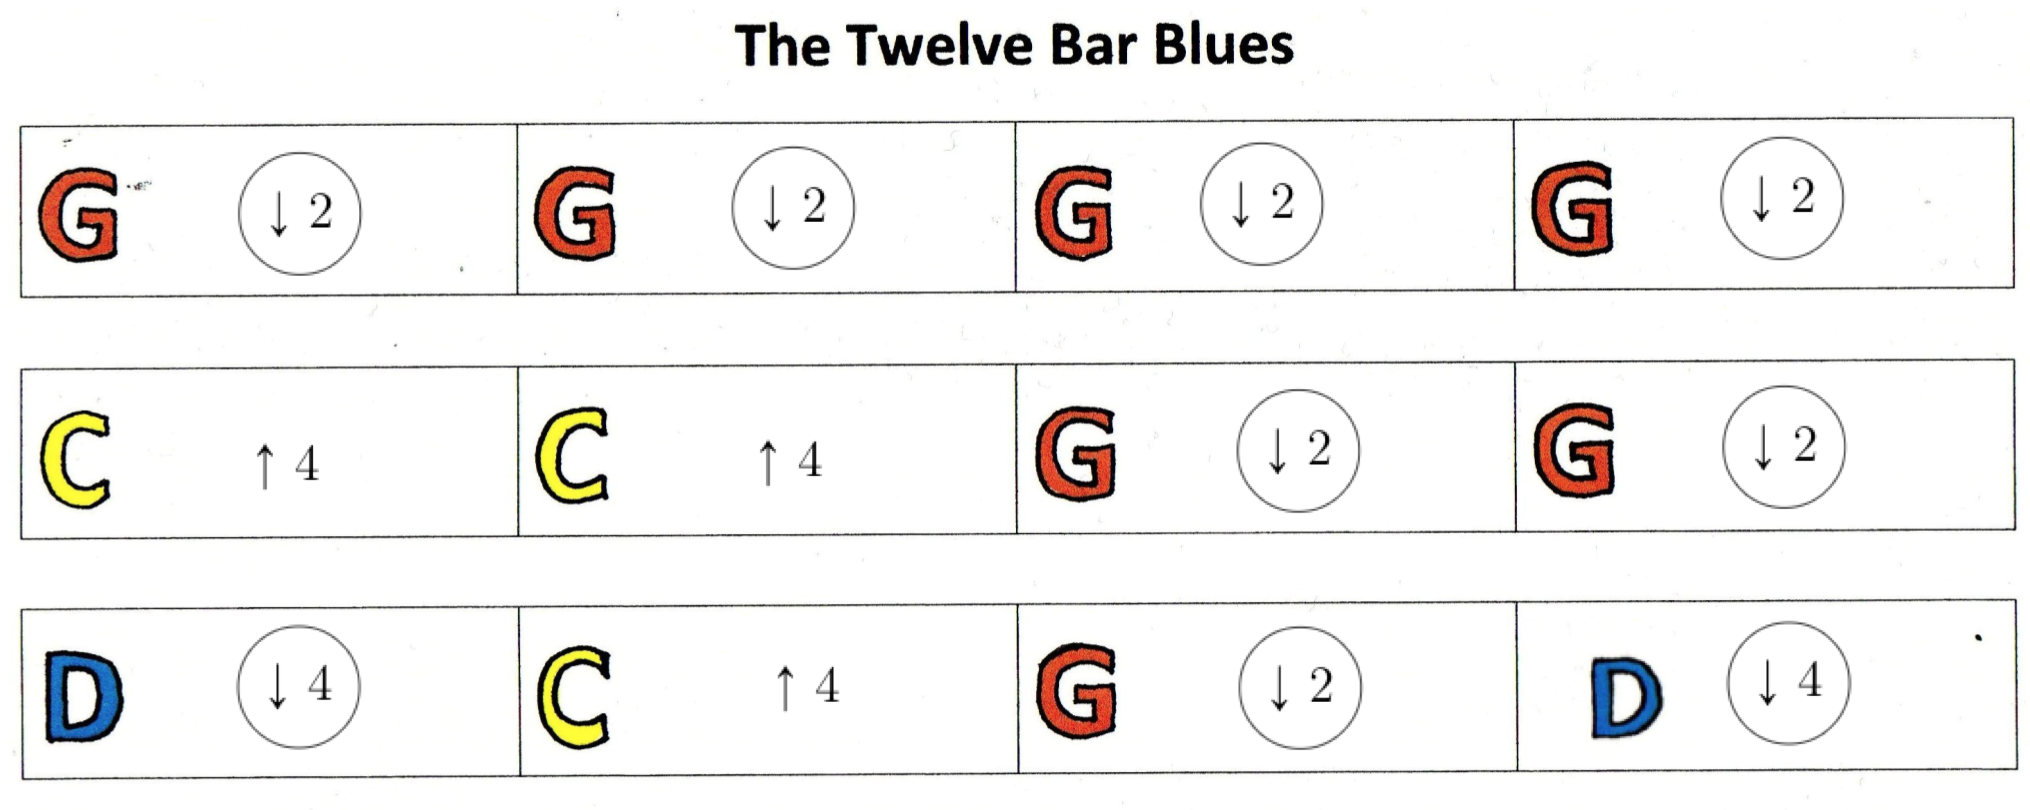
\includegraphics[scale=0.4]{12barbluesharmonica}
    



First practice just playing the root note. 
Then, play the root note of each chord at the start of the bar, then add notes from the blues scale to fill in the rest of the bar. You can add any of the riffs you have learned so far. 
(Spoiler: It's great to practice starting every bar with the root note, but it also doesn't matter if you don't play the root note all the time, as long as your playing revolves around the root note of the chord.)

\newpage    
    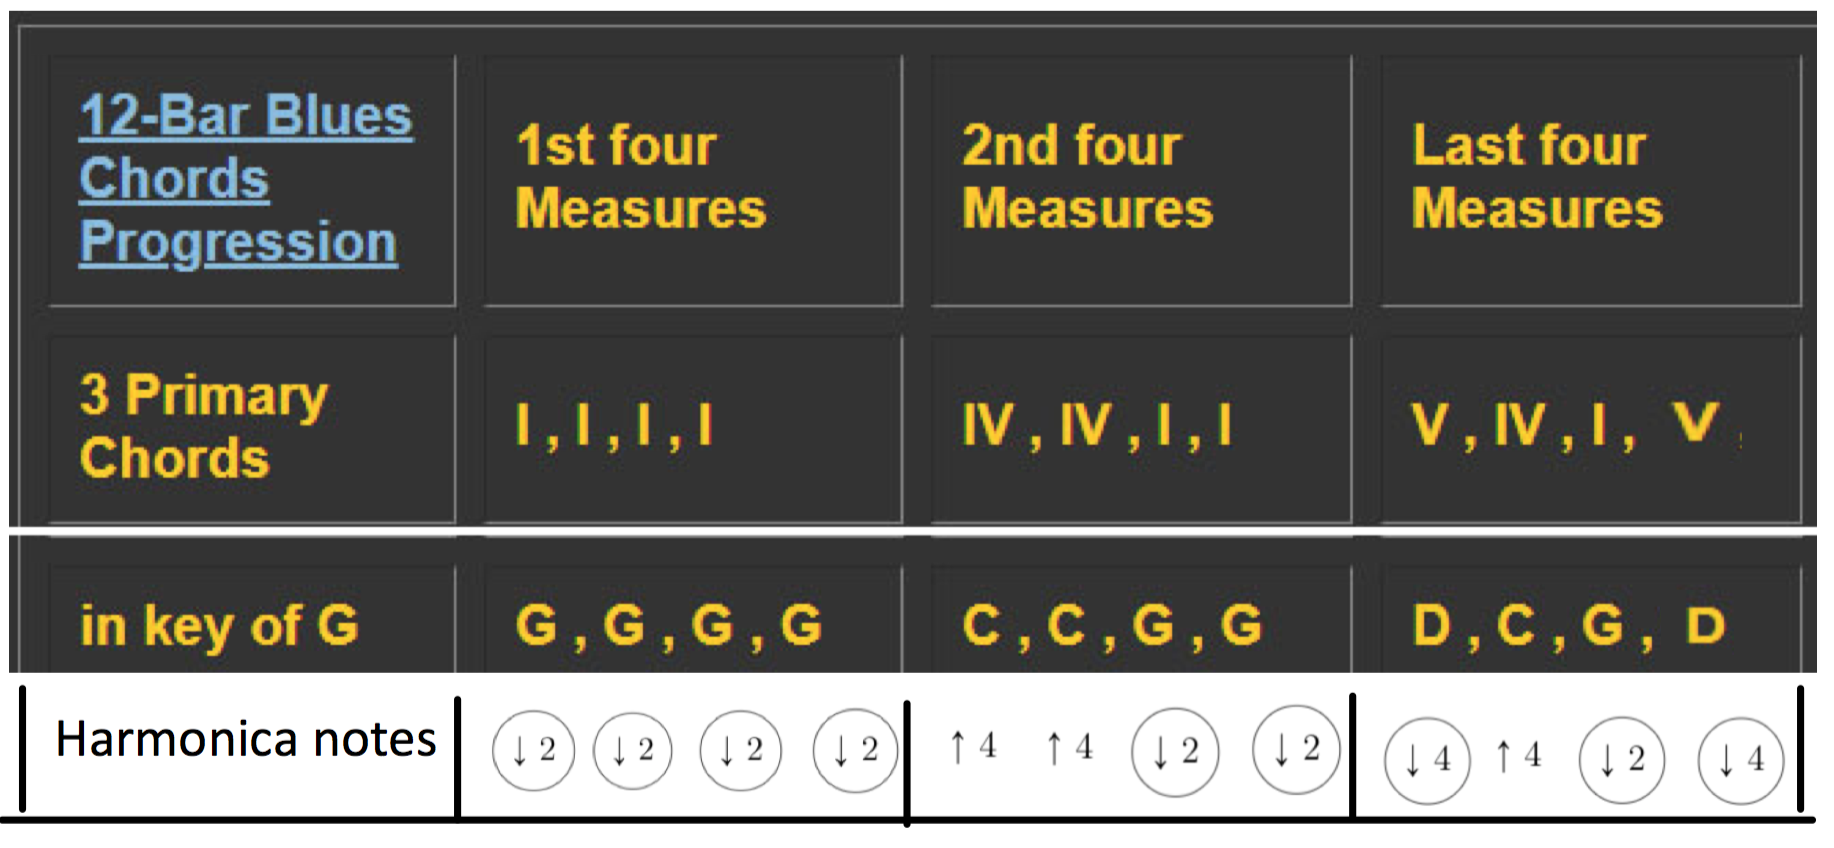
\includegraphics[scale=0.4]{12barbluesharmonica2}
\newpage
 \section{Blues scale}

\subsection{Going up - Main Octave}\\
\2\3\four\e\4\5\six\\

\subsection{Going down - Main Octave}\\
\six\5\4\e\four\3\2

\subsection{Going down (lower octave) - easy version}\\
\2\w\1\\


\subsection{Blues scale - most important notes (Going Up)}\\
\1\w \2 \\
\2\3\four\e\4\5\\

\subsection{Blues scale - most important notes (Going Down)}\\
\5\4\e\four\3\2 \\
\2\w\1\\





% \newpage

% \subsection{Blues scale - most important notes (Going Up)}\\
% \2\3\e\4\\\
